\chapter{VBF Varied Coupling Samples}\label{app:vbf-couplings}

In addition to the \gls{SM} VBF \hh sample used in Chapter~\ref{ch:vbf}, samples have been produced for the various coupling values shown in Table~\ref{tab:vbf-coupling-samples}. These samples were generated using the same generators and showering as described in Section~\ref{ssec:vbf-samples-production}. The values of $\kappa_\lambda$,$c_{2V}$, and $c_{v}$ are all 1 in the \gls{SM}. The values selected for production aim to vary each coupling value enough that interpolation may be performed, and one value was produced near where limits could be expected to be set ($\kappa_\lambda = 10$ and $c_{2V}=4$).

\begin{table}[htbp]
    \centering
    \caption{Grid of coupling values used in production of VBF $HH$ samples.}
    \begin{tabular}{c|c|c}
        $\kappa_\lambda$ & $c_{2V}$ & $c_{v}$ \\
        \hline
        1 & 0 & 0.5 \\
        1 & 1 & 0.5 \\
        0 & 0 & 1 \\
        1 & 0 & 1 \\
        1 & 0.5 & 1 \\
        1 & 0 & 0.5 \\
        1 & 1 & 1 \\
        1 & 1.5 & 1 \\
        1 & 2 & 1 \\
        1 & 4 & 1 \\
        0 & 1 & 1 \\
        2 & 1 & 1 \\
        10 & 1 & 1 \\
        1 & 1 & 1.5
    \end{tabular}
    \label{tab:vbf-coupling-samples}
\end{table}

Relevant distributions for validation of these samples can be seen in Figure~\ref{fig:vbf-mc-validation}. Plots are shown at parton level, with a basic jet selection applied to isolate the VBF jets similar to that done at reconstruction level. Jets are considered if they have $\pt > 25$, then the \mbb pair is selected as the two jets with \mbb closest to 125 \GeV. The VBF jets are selected as the highest $m_{jj}$ pair after removing jets used in the \mbb pairing. Additional detail on the validation for these samples is outlined in Reference~\cite{mc-validation}.

\begin{figure}[htbp]
    \centering
    \subfloat{
      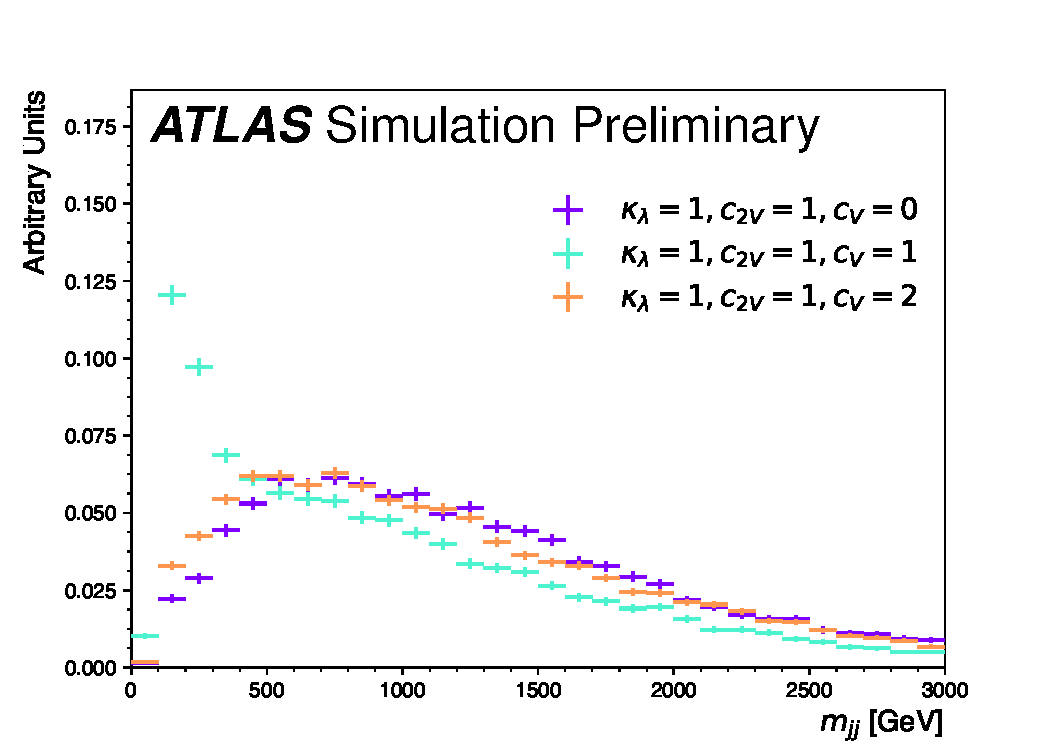
\includegraphics[width=0.33\textwidth]{chapters/chapter6_vbf/images/mc_samples/m_jj_cv.pdf}
    }
    \subfloat{
      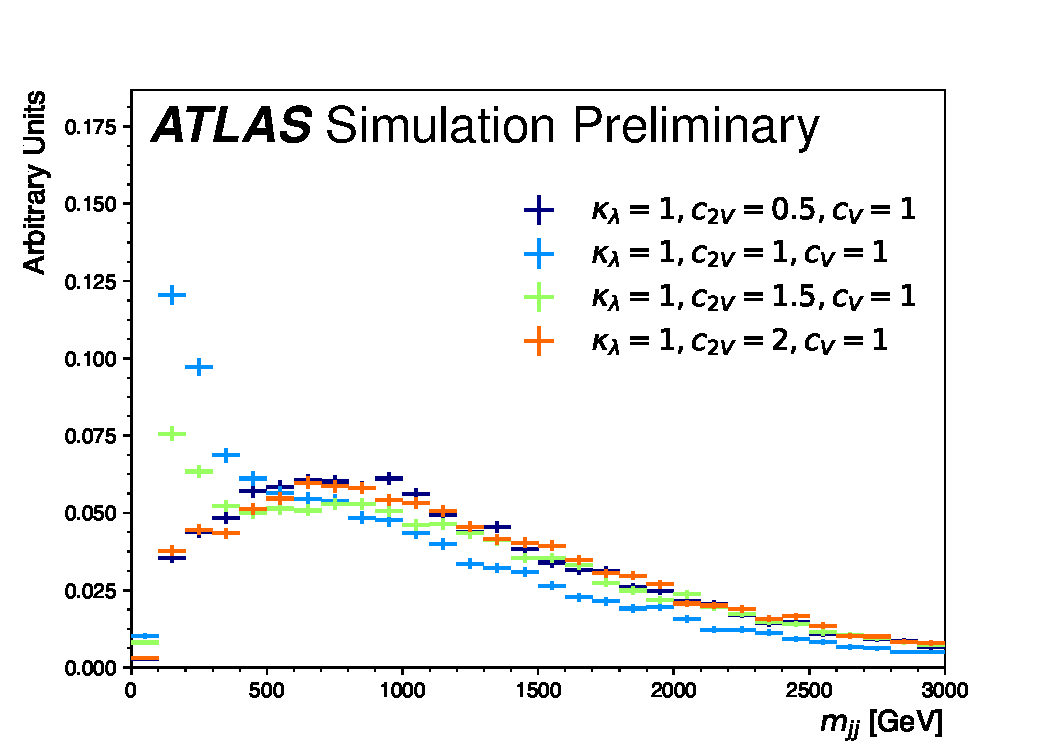
\includegraphics[width= 0.33\textwidth]{chapters/chapter6_vbf/images/mc_samples/m_jj_cvv.pdf}
    }
    \subfloat{
      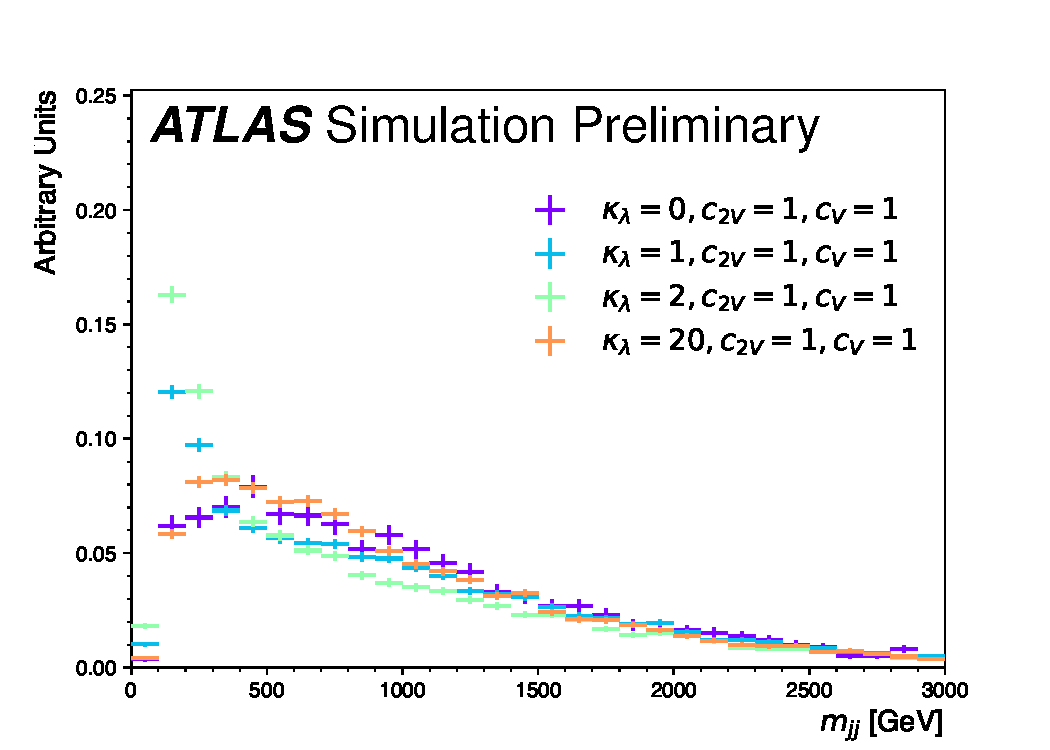
\includegraphics[width= 0.33\textwidth]{chapters/chapter6_vbf/images/mc_samples/m_jj_klambda.pdf}

    }       

    \subfloat{
        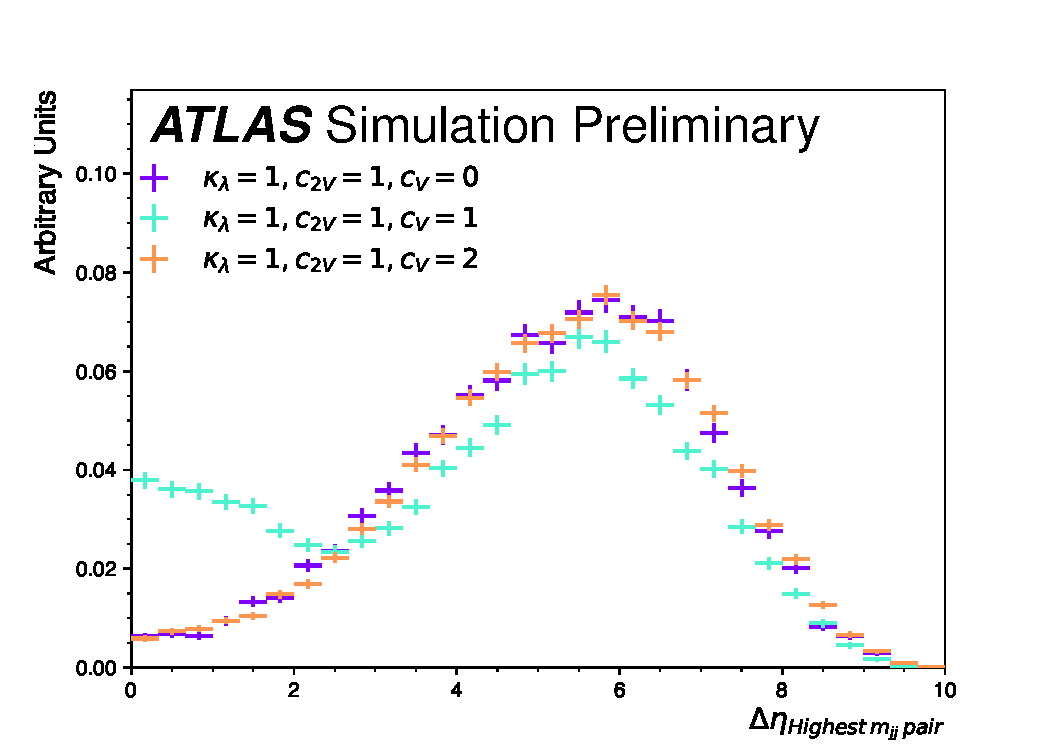
\includegraphics[width=0.33\textwidth]{chapters/chapter6_vbf/images/mc_samples/jj_deta_cv.pdf}
      }
      \subfloat{
        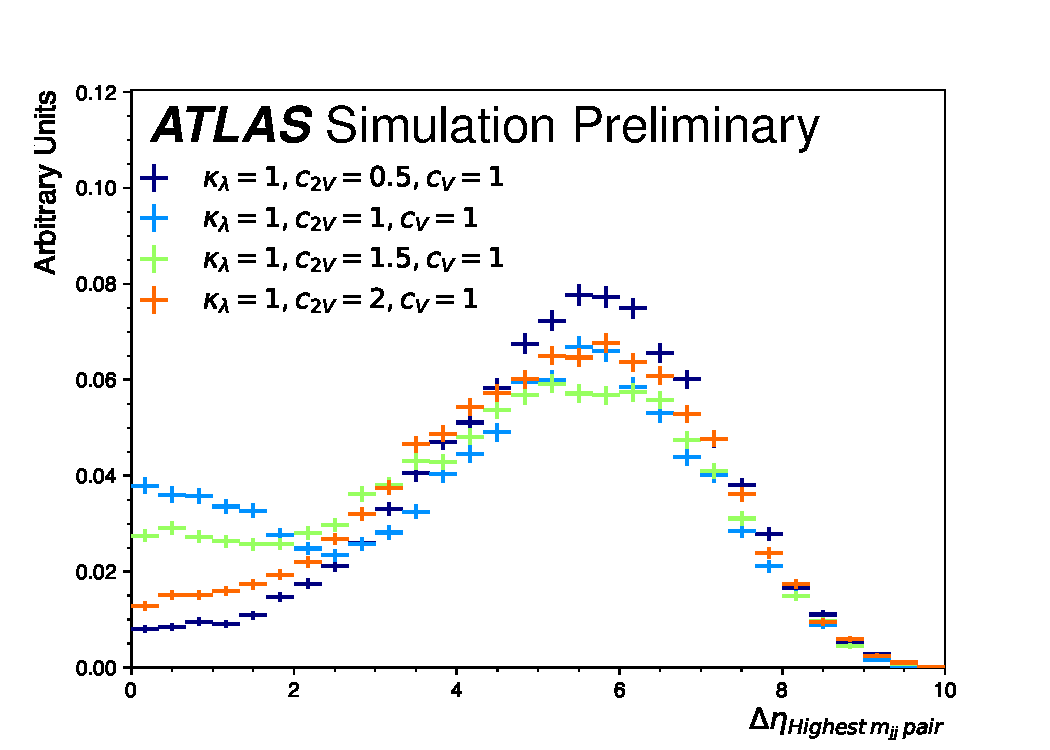
\includegraphics[width= 0.33\textwidth]{chapters/chapter6_vbf/images/mc_samples/jj_deta_cvv.pdf}
      }
      \subfloat{
        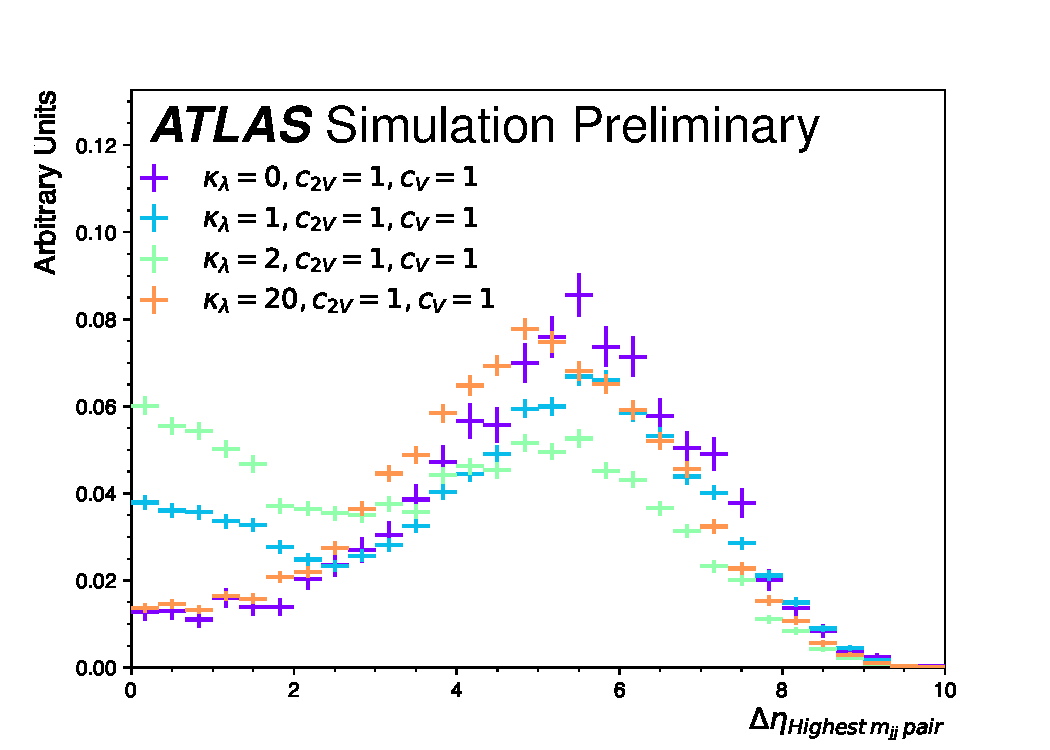
\includegraphics[width= 0.33\textwidth]{chapters/chapter6_vbf/images/mc_samples/jj_deta_klambda.pdf}
    }    

    \caption[Validation plots at parton level for the VBF \hh signal samples]{Validation plots at parton level for the VBF $HH$ signal samples. The highest $m_{jj}$ pair is selected as a proxy for the VBF jets. The top row shows the invariant mass distribution of this system, the bottom depicts the $\Delta \eta$ between these jets. Left to right, these plots vary the $c_V$, $c_{2V}$, and $\kappa_\lambda$ strength. The peak at low $m_{jj}$ values and shoulder at low $\Delta \eta$ is a product of the $VHH$ hadronic and Higgsstrahlung contributions in the samples.}
    \label{fig:vbf-mc-validation}
\end{figure}